% !!!IMPORTANT NOTE: Please read carefully all information including those preceded by % sign
%Before you compile the tex file please download the class file AIMS.cls from the following URL link to the
%local folder where your tex file resides. http://aimsciences.org/journals/tex-sample/AIMS.cls.
\documentclass{aims}
\usepackage{amsmath}
  \usepackage{paralist}
  \usepackage{graphics} %% add this and next lines if pictures should be in esp format
  \usepackage{epsfig} %For pictures: screened artwork should be set up with an 85 or 100 line screen
\usepackage{graphicx}  \usepackage{epstopdf}%This is to transfer .eps figure to .pdf figure; please compile your paper using PDFLeTex or PDFTeXify.
 \usepackage[colorlinks=true]{hyperref}
   % Warning: when you first run your tex file, some errors might occur,
   % please just press enter key to end the compilation process, then it will be fine if you run your tex file again.
   % Note that it is highly recommended by AIMS to use this package.

 %\usepackage{float}
\usepackage{booktabs,tabularx}
\usepackage[pagewise]{lineno}\linenumbers

\hypersetup{urlcolor=blue, citecolor=red}
%\usepackage{hyperref}

  \textheight=8.2 true in
   \textwidth=5.0 true in
    \topmargin 30pt
     \setcounter{page}{1}

% The next 5 line will be entered by an editorial staff.
\def\currentvolume{X}
 \def\currentissue{X}
  \def\currentyear{2019}
   \def\currentmonth{XX}
    \def\ppages{X--XX}
     \def\DOI{10.3934/xx.xx.xx.xx}

 % Please minimize the usage of "newtheorem", "newcommand", and use
 % equation numbers only situation when they provide essential convenience
 % Try to avoid defining your own macros

\newtheorem{theorem}{Theorem}[section]
\newtheorem{corollary}{Corollary}
\newtheorem*{main}{Main Theorem}
\newtheorem{lemma}[theorem]{Lemma}
\newtheorem{proposition}{Proposition}
\newtheorem{conjecture}{Conjecture}
\newtheorem*{problem}{Problem}
\theoremstyle{definition}
\newtheorem{definition}[theorem]{Definition}
\newtheorem{remark}{Remark}
\newtheorem*{notation}{Notation}
\newcommand{\ep}{\varepsilon}
\newcommand{\eps}[1]{{#1}_{\varepsilon}}


%% Place the running title of the paper with 40 letters or less in []
 %% and the full title of the paper in { }.
\title[a model of tumor-immune system interaction] %Use the shortened version of the full title
      {Dynamics of a Model of Tumor-Immune Interaction with Time Delay and Noise}

% Place all authors' names in [ ] shown as running head, Leave { } empty
% Please use `and' to connect the last two names if applicable
% Use FirstNameInitial.  MiddleNameInitial. LastName, or only last names of authors if there are too many authors
\author[Lifeng Han, Changhan He and Yang Kuang]{}

% It is required to enter 2010 MSC.
\subjclass{34D05, 34D20, 92D25.}
% Please provide minimum  5 keywords.
 \keywords{time delay, stochasticity, persistence, stability, tumor-immune interaction}

% Email address of each of all authors is required.
% You may list email addresses of all other authors, separately.
 \email{lifeng.han@asu.edu}
 \email{changhan.he@asu.edu}
 \email{kuang@asu.edu}

% Put your short thanks below. For long thanks/acknowledgements,
%please go to the last acknowledgements section.
\thanks{The authors are supported by NSF grant 161587 and NIH grant 1R01GM131405-01}

% Add corresponding author at the footnote of the first page if it is necessary. 
% Please add $^*$ adjacent to the corresponding author's name on the first page. 
% The example shown in this template is if the first author is the corresponding author.
\thanks{$^*$ Corresponding author: Yang Kuang}




\begin{document}
\maketitle

% Enter the first author's name and address:
\centerline{\scshape Lifeng Han, Changhan He and Yang Kuang $^*$}
\medskip
{\footnotesize
% please put the address of the first author
 \centerline{School of Mathematical and Statistical Sciences}
   \centerline{Arizona state University}
   \centerline{Tempe, AZ 85287-1804, USA}
} % Do not forget to end the {\footnotesize by the sign }

%\medskip
%
%\centerline{\scshape First-name2 last-name2 and First-name3
%last-name3}
%\medskip
%{\footnotesize
% % please put the address of the second  and third author
% \centerline{ First line of the address of the second author}
%   \centerline{Other lines}
%   \centerline{Springfield, MO 65810, USA}
%}

\bigskip

% The name of the associate editor will be entered by an editorial staff
% "Communicated by the associate editor name" is not needed for special issue.
 \centerline{(Communicated by the associate editor name)}



\begin{abstract}
We propose a model of tumor-immune interaction with time delay in immune reaction and noise in tumor cell reproduction. Immune
response is modeled as a non-monotonic function of tumor burden, for
which the tumor is immunogenic at nascent stage but starts inhibiting
immune system as it grows large. Without time delay and noise, this system demonstrates bistability.
The effects of response time of the immune system and uncertainty
in the tumor innate proliferation rate are studied by including delay
and noise in the appropriate model terms. Stability, persistence
and extinction of the tumor are analyzed. We find that delay
and noise can both induce the transition from low tumor burden equilibrium
to high tumor equilibrium. Moreover, our result suggests that the elimination of cancer depends on the basal level of the immune system rather than on its response speed to tumor growth.
\end{abstract}


\section{Introduction}

The immune system is a host defense system that distinguishes pathogens from one's own healthy cells and destroy them. Pathogens include bacteria and viruses as well as abnormal cells. There are evidence that immune systems can detect and eliminate cancer \cite{parish2003cancer}. Cancer immunology has seen renewed interests due to recent achievements in immunotherapy \cite{mahoney2015next}. Unlike common pathogens, cancer cells are not as distinguishable. Moreover, cancer can evade the control of immune systems by developing ways to achieve immune suppression \cite{Whiteside2006}. Recent progress in immunotherapy has focused on removing immune suppression so that cancer cells will be under attack of immune systems. Further development of immunotherapy hinges on a better understanding of tumor-immune system interaction. 

The immune system consists of immune cells of several types and complex
signaling network. For example, immune cells include cytotoxic T cells,
helper cells, natural killer cells, and signaling networks involve
cytokines, e.g., interlukin-2. The immune response falls into two
categories: innate and adaptive. Though the adaptive response enables
fast reaction to certain antigens, immune responses oftentimes involve
recruiting immune cells from bone marrows and further training or
activation. So it is inherently a delayed process. On the other hand,
cancer is well-known for its heterogeneity and characterized by fast
mutation, which can render it the ability to suppress immune response
\cite{fisher2013cancer,Whiteside2006}. In this process, stochasticity
plays an important role. 

Given the complexity of tumor-immune system interaction, mathematical
modeling naturally offers some insights by capturing the key mechanisms.
Literature on modeling non-spatial tumor growth under immune surveillance
is abundant (see \cite{Eftimie2011} for a review). In \cite{Kuznetsov1994},
the authors derived a system of five equations from a kinetic scheme
and further reduced it to two equations tracking only effector cells
and tumor cells. In their model, immune suppression is represented
as annihilation by mass action of tumor cells and effector cells.
Their paper inspired a number of later work. In \cite{dOnofrio2008},
the author summarized models of this type into a family as follows\begin{subequations}\label{eq: dOnofrio}
\begin{eqnarray}
x' & = & x(f(x)-\phi(x)y),\\
y' & = & -\Psi(x)y+\sigma q(x)+\theta(t)
\end{eqnarray}
\end{subequations} where $x$ is the size or density of tumor population,
$y$ is the size or density of immnue effector population and $\theta(t)$
represents treatment . With biological-relevant assumptions on $f(x),\phi(x)$
and $q(x)$, some general conclusions of were drew in \cite{dOnofrio2008}. 

In \cite{Kirschner1998}, the authors took into account cytokines
in their model in order to gain further insight into immunotherapy.
In most cases, introducing more equations does not introduce new dynamics
but is necessary to shed light on cancer treatments \cite{Eftimie2011}.
Signaling is arguably a fast process, so sometimes a quasi-steady
state approximation can reduce more complicated models into the family
of models studied by \cite{dOnofrio2008}. For example, in a recent
study on immune check point inhibitor \cite{Nikolopoulou2018}, a
variation of (\ref{eq: dOnofrio}) is derived from a more complicated
model consisting of a system of 14 partial differential equations
\cite{Lai2017}. 

Building on aforementioned earlier work, the effect of time delay
in tumor-immune interactions are also extensively studied \cite{Banerjee2008,dOnofrio2010,galach2003dynamics,Rihan2014}.
On the other hand, stochasticity in tumor-immune interaction is less
often studied, and mostly focused on single-equation models of tumor
population growth ignoring explicit interaction with immune system
\cite{Lefever1979,Bose2009,Li2017}. Models that take into account
both time delay and stochasticity are even rarer. To the best of our
knowledge, the work of \cite{Guo2014} is the only exception. In \cite{Guo2014},
a single equation was considered and noise was introduced in an ad-hoc
way. To fill this gap, we will introduce time delay and noise one
at a time to a variation of (\ref{eq: dOnofrio}) with the novelty
in its immune response term being non-monotonic. 

The paper is organized as follows. In section 2, we introduce our
model formulation and state general properties of the model in absence
of noise and time delay. In section 3, we study the model with time
delay where persistence, local stability and global stability results
are presented. Section 4 is devoted to the stochastic version of the
model where tumor extinction and persistence conditions are presented.
In section 5, the paper comes to the culmination where both noise
and time delay are present in the model, for which we study the effects
of time delay on the stationary distribution. We conclude the paper
with a discussion of future work in section 6. 

\section{ODE model formulation and properties }

We consider the following equations 

\begin{eqnarray}
\frac{dx}{d\hat{t}} & = & \hat{\rho}x(1-\frac{x}{\hat{K}})-\hat{\gamma}xy,\\
\frac{dy}{d\hat{t}} & = & \hat{\beta}-\hat{\mu}y+\frac{\hat{\alpha}x}{\hat{\kappa}+x^{2}},
\end{eqnarray}
 where $x$ denotes the tumor burden and $y$ denotes the level of
immune response. This is a special case of (\ref{eq: dOnofrio}) for
which we specify $\sigma q(x)=\hat{\beta}+\frac{\hat{\alpha}x}{\hat{\kappa}+x^{2}}$
to represent the immune response to tumor burden in a non-monotonic
fashion. In spite of being phenomenological, it accounts for the fact
that the cancer cells acquire mutations that can down-regulate immune
response as the tumor grows bigger while the tumor is immuogenic at
its nascent stage. Death term is assumed to be independent of tumor
burden and thus we have $\Psi(x)y=-\hat{\mu}y$. Note that without
tumor, immune system activity is maintained at the basal level $\beta/\mu$.
We assume logistic growth of tumor and that killing of tumor cells
by the immune system is represented as a mass action term so that
we have $f(x)=1-\frac{x}{\hat{K}}$ and $\phi(x)=\hat{\gamma}x$.
Both are common choices in modeling literature \cite{galach2003dynamics,Nikolopoulou2018}.
Even though Gompertz growth is also commonly used in modeling tumor
growth and backed up by a lot of experimental data, it predicts unbound
growth rate as tumor burden approaches zero \cite{Eftimie2011}. Hence
it is not suitable to our purpose. 

Note that we represent the two populations generically as tumor burden
and level of immune response, and intentionally avoid using specific
units of cell density or volume. In some sense, it justifies our choice
of $\Psi(x)y=-\hat{\mu}y$ since we are not tracking explicitly effector
cells. The rationale behind our generic representation is that our
objective is to study interesting dynamics that can arise from a simple
model with time delay and noise. It is our intention to bring attention
to the possible key mechanisms underlying cancer-immune system dynamics
without making the wrong impression that it is capable of clinical
prediction. 

By nondimensionlization, we can reduce the number of parameters. Let
$x=\sqrt{\kappa}u$, $y=\frac{\alpha}{\mu\sqrt{\kappa}}v$ and $t=\frac{1}{\mu}\hat{t}$.
We get the dimensionless system 

\begin{subequations}\label{eq: uv }
\begin{align}
\frac{du}{dt} & =\rho u(1-\frac{u}{K})-\gamma uv\equiv f(u,v),\\
\frac{dv}{dt} & =\beta-v+\frac{u}{1+u^{2}}\equiv g(u,v).
\end{align}
\end{subequations} where $\rho=\frac{\hat{\rho}}{\hat{\mu}},\,K=\frac{\hat{K}}{\sqrt{\hat{\kappa}}},\,\gamma=\frac{\hat{\alpha}\hat{\gamma}}{\hat{\mu}^{2}\sqrt{\hat{\kappa}}}$ and $\beta=\frac{\hat{\beta}\sqrt{\hat{\kappa}}}{\hat{\alpha}}$ are dimensionless (positive) parameters.
It can be shown that there is always a tumor free equilibrium $E_{0}=\{0,\beta\}$
which is stable if and only if $\rho<\gamma\beta$ by linear stability analysis.
If $\rho>\gamma \beta$, depending on the parameters, there is additional either one or three interior
equilibria. In this paper, we focus on the case where there are
three interior equilibria, namely low tumor equilibrium $E_{1}$, intermediate tumor equilibrium $E_{2}$ and high tumor equilibrium $E_{3}$
(see Figure \ref{fig:Nullclines}). Since the intersections of nullclines
are roots of a cubic polynomial, any results involving analytical
expressions of parameters for stability conditions, if possible, would
be unwieldy. Nevertheless, qualitative argument similar to that of in (\cite{murraymathematical} P226-230) can be made regarding to the local stability .
By doing so, we obtain the theorem below.
\begin{theorem} \label{thm:ODE local stability}
Suppose that $\rho>\gamma\beta$ and there are three interior equilibria $E_1,E_2$ and $E_3$ of (\ref{eq: uv }), then $E_1$ and $E_3$ are stable, and $E_2$ is unstable.   
\end{theorem}
\begin{proof}
Consider the Jacobian matrix at the equilibrium 
\[
J=\begin{bmatrix}
f_u & f_v\\
g_u & g_v
\end{bmatrix}
\]
where $f_{u},f_{v},g_{u}$ and $g_{v}$ are the partial derivatives of $f(u,v)$ and $g(u,v)$ evaluated at the equilibrium. The signs of $f_{u},f_{v},g_{u}$ and $g_{v}$ can be determined by geometric arguments. For example, to see the sign of $g_{u}$ at $E_1$, we first note that $g(u,v)<0$ in the region above $g(u,v)=0$ and $g(u,v)<0$ in the region below. Thus as it moves across $g(u,v)=0$ at $E_1$ along the direction of $u$-axis from left to right, $g(u,v)$ increases from being negative to being positive. Therefore, $g_u>0$ at $E_1$. By the same argument, we find out the signs of the entries of Jacobian matrices $J_1$, $J_2$ and $J_3$ at $E_1,E_2$ and $E_3$ as follows
\begin{eqnarray} \label{eq:J}
J_{1}=\begin{bmatrix}- & -\\
+ & -
\end{bmatrix} & J_{2}=\begin{bmatrix}- & -\\
- & -
\end{bmatrix} & J_{3}=\begin{bmatrix}- & -\\
- & -
\end{bmatrix}
\end{eqnarray}
Thus $Tr(J_1)<0, Tr(J_2)<0$ and $Tr(J_3)<0$. To determine stability, we need to find signs of their determinants too. This can be done by noting the sign of the slopes of the nullclines. For example, at $E_1$, $\frac{dv}{du}>0$ along $g(u,v)=0$ and $\frac{dv}{du}<0$ along $f(u,v)=0$. Implicit differentiating $g(u,v)=0$ with respect to $u$ gives $\frac{dv}{du}=-\frac{g_u}{g_v}$. Similarly, we have $\frac{dv}{du}=-\frac{f_u}{f_v}$ along $f(u,v)=0$. Hence at $E_1$, we have $-\frac{g_u}{g_v}>0>-\frac{f_u}{f_v}$. Since $g_v<0,f_v<0$ at $E_1$, $\det(J_1)=f_u g_v - f_v g_u>0$. Similarly, we have $\det(J_2)<0$ and $\det_(J_3)>0$. Therefore, we proved the claimed stability.      
\end{proof}

\begin{figure}[tph]
\begin{centering}
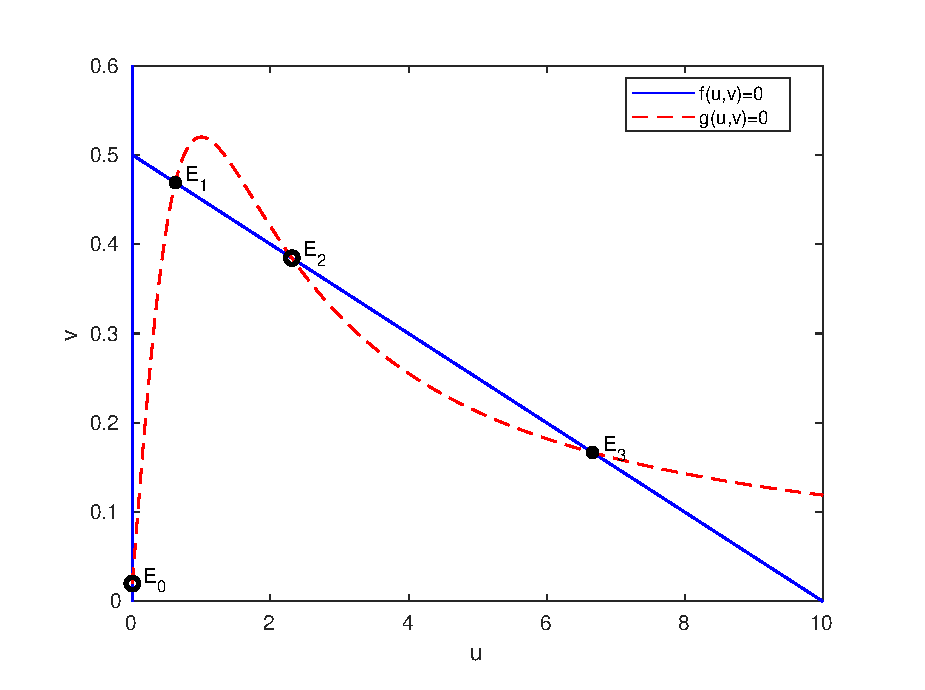
\includegraphics[scale=0.6]{explore/plots/nullclines/nullclines-new}
\par\end{centering}
\caption{\label{fig:Nullclines}Nullclines of (\ref{eq: uv }). Open circles
denote unstable fixed points and filled circle denotes stable fixed
points. Parameter values used: $\rho=2.5,\text{\ensuremath{\beta=0.02,\gamma=5,K=10}}$ }
\end{figure}


\section{With delay}

It is known that it takes time for the immune system to respond and
take effect. So we introduce time delay into the term representing
immune response. The model now reads as follows 

\begin{subequations}\label{eq:main delay}
\begin{align}
u' & =\rho u(1-\frac{u}{K})-\gamma uv\\
v' & =\beta-v+\frac{u(t-\tau)}{1+u(t-\tau)^{2}}.
\end{align}
\end{subequations}
where $\tau \ge 0$ is the time delay of immune response. We are curious about any possible new dynamics due to the time delay in contrast to the ODE model, especailly if the time delay in immune response can lead to oscillatory solutions that may represent cancer growth episodes. 

\subsection{Analysis}
First we want to establish positivity and boundedness of the system (\ref{eq:main delay}) given appropriate initial values. For initial values, we assume $v(0) \ge 0$ and $u(\theta) = \phi(\theta)$ for $\theta \in [-\tau,0]$ where $\phi(\theta) \in C([-\tau,0]): \phi(\theta) \ge 0$ and $\phi(0)>0$.

\begin{proposition} \label{prop:bdd}
The solution of (\ref{eq:main delay}) satisfies that $u(t) > 0$ and $v(t) > 0$ for all $t>0$. Moreover, $\limsup_{t\to\infty}u(t) \le K$ and $\beta \le \liminf_{t\to\infty} v(t) \le \limsup_{t\to\infty} v(t) \le \beta+1/2$. 
\end{proposition}
\begin{proof}
Suppose there exists $t_1>0$ such that $u(t_1)=0$ and $u(t)>0$ for $t \in (0,t_1)$. Note that (\ref{eq:main delay}a) is in the form $u'=u F(u,v)$. Then $$u(t_1)=u(0) \exp (\int_0^{t_1} F(u(s),v(s)ds)>0,$$ which is a contradiction. The positivity of $v$ is obvious as if there is $t_1$ such that $v(t_1)=0$, then $v'(t_1)>0$. The boundedness is straightforward.
\end{proof}

The above proposition ensures that the solution of (\ref{eq:main delay}) is biological meaningful and will also be useful prerequisite for our later analysis. Next we present a theorem of the local stability of (\ref{eq:main delay}) as a counterpart to Theorem \ref{thm:ODE local stability}. In particular, we show that as $\tau$ increases there is a possible stability switching for low tumor equilibrium $E_1$. Recalling the same definition for $f_{u},f_{v},g_{u}$ and $g_{v}$ as before, we have the following theorem. 

\begin{theorem}
Suppose that $\rho>\gamma\beta$. Then the tumor free equilibrium $E_0$ is unstable for for all $\tau \ge 0$. In addition, suppose that there are three interior equilibria $E_1,E_2$ and $E_3$ of (\ref{eq:main delay}). Then $E_3$ is stable, $E_2$ is unstable for all $\tau \ge 0$ and $E_1$ change its stability as $\tau$ increases if $f_{u}g_{v}+f_{v}g_{u}<0$.
\end{theorem}

\begin{proof}
Linearizing (\ref{eq:main delay}) at the equilibrium gives
\begin{eqnarray*}
u' & = & f_{u}u+f_{v}v\\
v' & = & g_{u}u(t-\tau)+g_{v}v
\end{eqnarray*}
Substituting $u=Ae^{\lambda t},v=Be^{\lambda t}$
into the above equations yields a linear system of $A$ and $B$ for
which the existence of a solution entails the characteristic equation
\begin{equation}
\lambda^{2}-(f_{u}+g_{v})\lambda+f_{u}g_{v}-f_{v}g_{u}e^{-\lambda\tau}=0.\label{eq:chara eqn}
\end{equation}
At $E_0$, (\ref{eq:chara eqn}) becomes $\lambda^2-(\rho-\gamma\beta)\lambda-\rho+\gamma\beta=0$, which always has a positive root and thus $E_0$ remains unstable for all $\tau\ge0$.

Theorem \ref{thm:ODE local stability} gives the stability results of $E_1$, $E_2$ and $E_3$ at $\tau=0$. We want to study if their stability changes as time delay $\tau$ increases. If the equilibrium changes its stability as $\tau$ increases, there must exists $\omega>0$ such that $\lambda=i\omega$ is a solution of (\ref{eq:chara eqn}) \cite{KuangDDEBook}. Substituting $\lambda=i\omega$ into (\ref{eq:chara eqn}) gives 
\[
-\omega^{2}-(f_{u}+g_{v})(i\omega)+f_{u}g_{v}-f_{v}g_{u}(\cos(\omega\tau)-i\sin(\omega\tau))=0.
\]
Collecting real and imaginary parts gives
\[
(f_{u}g_{v}-\omega^{2}-f_{v}g_{u}\cos(\omega\tau))-((f_{u}+g_{v})\omega+f_{v}g_{u}\sin(\omega\tau)i=0.
\]
Equating the real and imaginary parts to zeros respectively gives
\begin{subequations}\label{eq: cos sin}
\begin{eqnarray}
\cos(\omega\tau) & = & \frac{f_{u}g_{v}-\omega^{2}}{f_{v}g_{u}},\\
\sin(\omega\tau) & = & -\frac{(f_{u}+g_{v})\omega}{f_{v}g_{u}}.
\end{eqnarray}
\end{subequations} Squaring and adding the above equations gives
\[
\omega^{4}+(f_{u}^2+g_{v}^2)\omega^{2}+f_{u}^{2}g_{v}^{2}-f_{v}^{2}g_{u}^{2}=0
\]
which has a real solution $\omega=\omega_{0}$ if and only if 
\begin{equation}
(f_{u}g_{v}-f_{v}g_{u})(f_{u}g_{v}+f_{v}g_{u})<0.\label{eq:real omega ineq}
\end{equation}
From (\ref{eq:J}), we see that (\ref{eq:real omega ineq}) is not satisfied for $E_{3}$ and hence it has no stability switching. Stability switching is possible for $E_1$ and $E_2$.
For $E_{1}$, (\ref{eq:real omega ineq}) entails an additional requirement 
\begin{equation}
f_{u}g_{v}+f_{v}g_{u}<0, \label{eq:swtiching cond}
\end{equation} 
which is stated in the theorem. 
The critical value of $\tau$ can be found
by substituting $\omega=\omega_{0}$ to (\ref{eq: cos sin}), which
leads to 
\[
\tau_{0}=\frac{1}{\omega_{0}}[\arctan(\frac{f_{u}g_{v}-\omega_{0}^{2}}{(f_{u}+g_{v})\omega_{0}})].
\]
To ensure stability switching, We need further confirm that the imaginary
root crosses the imaginary axis as $\tau$ increases beyond $\tau_{0}$.
To do so, we think $\lambda$ as a function of $\tau$ and differentiating
(\ref{eq:chara eqn}) gives 
\begin{eqnarray*}
[2\lambda-(f_{u}+g_{v})+f_{v}g_{u}e^{-\lambda\tau}\tau]\frac{d\lambda}{d\tau} & = & -f_{v}g_{u}e^{-\lambda\tau}\lambda.
\end{eqnarray*}
 It follows that 
\begin{eqnarray*}
\text{sgn}\bigg\{\bigg[\frac{d\Re(\lambda)}{d\tau}\bigg]_{\tau=\tau_{0}}\bigg\} & = & \text{sgn}\bigg\{\Re\bigg[(\frac{d\lambda}{d\tau})^{-1}\bigg]_{\tau=\tau_{0}}\bigg\}\\
 & = & \text{sgn}\bigg\{\frac{(f_{u}-g_{v})^{2}+2\omega_{0}^{2}}{f_{v}^{2}g_{u}^{2}}\bigg\}=1.
\end{eqnarray*}
So for $E_1$ which is stable at $\tau=0$, the imaginary root indeed crosses the imaginary axis and stability switching is ensured. But for $E_2$ which is unstable at $\tau=0$, the imaginary root does not cross the imaginary axis and there is no change in its stability.  
\end{proof}

The above theorem indicates that the time delay in immune response can lead to tumor escaping the control of the immune system as a consequence of loss of stability of the low tumor equilibrium.  The condition (\ref{eq:swtiching cond}) for this stability switching is not explicit in terms of parameters. Nevertheless, it has a geometric interpretation that the slope of the $v$-nullcine is larger than the magnitude of the slope of $u$-nullcline at their interception $E_{1}$. In a biological sense, it means that there would be instability if the objective of immune response level is set to increase steeply with respect to tumor burden while immune response time is not fast enough to catch up.

Next we study the global stability of the tumor free equilibrium. 
\begin{theorem}
\textup{(global stability of tumor free equilibrium)} 

If $\rho<\gamma\beta$, then $\lim_{t\to\infty}(u(t),v(t))=(0,\beta)$ 
\end{theorem}

\begin{proof}
We first shift $v$ to make its equilibrium value to be zero by letting $w=v-\beta$. We consider
the equivalent equation as below
\begin{eqnarray*}
u' & = & u(\rho-\gamma\beta-\frac{\rho u}{K}-\gamma w),\\
w' & = & -w+\frac{u(t-\tau)}{1+u(t-\tau)^{2}}.
\end{eqnarray*}
Assuming $\rho<\gamma\beta$, then there exists a $p$ such that  $\rho-\gamma\beta\ge p>0$.
Define 
\begin{eqnarray*}
V & = & \frac{1}{8p}u(t)^{2}+\frac{1}{2}w(t)^{2}+\frac{1}{4}\int_{t-\tau}^{t}u(s)^{2}ds.
\end{eqnarray*}
 It follow that 
\begin{eqnarray*}
\dot{V} & = & \frac{1}{4p}u(t)^{2}(\rho-\gamma\beta-\frac{\rho}{K}u-\gamma w)+w(-w+\frac{u(t-\tau)}{1+u(t-\tau)^{2}})\\
&  & +\frac{1}{4}(u(t)^{2}-u(t-\tau)^{2}) \\
 & = & (\frac{\rho-\gamma\beta}{4p})u(t)^{2} - \frac{\rho}{4pK}u(t)^3 - \frac{\gamma}{4p}wu(t)^2 \\
 &	& -w^2-\frac{1}{4}u(t-\tau)^2+\frac{wu(t-\tau)}{1+u(t-\tau)^2}.
\end{eqnarray*}
By construction, we have $\frac{\rho-\gamma\beta}{4p}<0$ and by Proposition \ref{prop:bdd}, we have $w=v-\beta \ge 0$ Hence, 
\[\
\dot{V} \le -(w-\frac{1}{2}u(t-\tau))^2 - \frac{\rho}{4pK}u(t)^3 \le 0
\]  
We also note that $\dot{V}=0$ if and only if $u(t)$ is identically zero and $w=u(t-\tau)/2$ which implies that $w$ must also be identically zero. Thus $\lim_{t\to\infty}(u(t),v(t))=(0,\beta)$
by Liapunov-LaSalle theorem (see \cite{KuangDDEBook} Theorem 2.5.3). 
\end{proof}
If the stability condition of tumor-free equilibrium is not satisfied,
we can prove that the tumor population is persistent. 
\begin{theorem} \label{thm:delay persistence}
\textup{(tumor persistence)} If $\rho>\gamma\beta$, there is $m>0$
such that \\
 $\limsup_{t\to\infty}u(t)>m$.
\end{theorem}

\begin{proof}
Suppose not. Then $\lim_{t\to\infty)} u(t)=0$. From this, it can be shown that $\limsup_{t\to\infty} v(t) \leq \beta$.  There are two cases we need to consider. The first case
is that $u$ is eventually monotonically decreasing to zero. Then
$\lim_{t\to\infty}v(t)=\beta$. It follows that there is a $t^{*}>0$
such that  $u(t^{*})$ is sufficiently small and $v(t^{*})$ is sufficiently close to $\beta$ so that
$u'(t^{*})=u(\rho-\frac{\rho u}{K}-\gamma v)>0$. So we have a contradiction.
The second case is that $u$ approaches zero in an oscillatory fashion.
That is, there is a sequence of $\{t_{i}\}$ such that $u(t_{i})\to0$
and $u(t_{i})$ is local minimum, i.e., $u'(t_{i})=u(\rho-\frac{\rho u}{K}-\gamma v)=0$.
Then for any $\delta>0$ there is an $N(\delta)$ such that  $u(t_{i})<\delta$
for $i>N(\delta)$. Since $\rho>\gamma \beta$, there is a $\delta$ such that $\rho-\frac{\rho\delta}{K}-\gamma(\beta+\delta)>0$. We see that for this $\delta$, there is a $T_1$ such taht $t>T_1$ implies that $v(t)<\beta + \delta$ and an $N$ such that for $i>N$, $t_i>T_1$. Hence for $i>N$, $u'(t_i)>0$ which is a contradiction to $u'(t_i)=0$.  
\end{proof}
Putting the conditions of the above two theorems in original units,
we find an important dimensionless value $R_0=\frac{\hat{\rho}\hat{\mu}}{\hat{\gamma}\hat{\beta}}$.
It is the ratio of the proliferation ability of
the tumor verse the strength of the immune system, which can be viewed as the tumor reproduction number: if 
\begin{equation}
R_0=\frac{\hat{\rho}\hat{\mu}}{\hat{\gamma}\hat{\beta}}<1,\label{eq:rhogammabeta}
\end{equation}
 the tumor can be totally cleaned out by immune system. The biological meaning of  (\ref{eq:rhogammabeta}) is more clear by recognizing that it is equivalent to saying that at the onset of tumor growth, the killing rate of tumor by the immune system ($\hat{\gamma} \hat{\beta} / \hat{\mu}$) is larger than the tumor growth rate ($\hat{\rho}$). Theorem \ref{thm:delay persistence} tells us that otherwise ($R_0>1$) the tumor will always exist. 

\subsection{Numerical simulation}

We studied (\ref{eq:main delay}) numerically using dde23 in Matlab.
We confirmed the criteria for tumor persistence and extinction in
our numerical experiment. The existence of a stability switching for
low tumor equilibrium as $\tau$ increases is also demonstrated (Figure
\ref{fig:stablity switch and shift}). Moreover, we discovered that
as $\tau$ is further increased, there is a transition to high
tumor equilibrium (bottom right of Figure \ref{fig:stablity switch and shift}).
Interestingly, the jerky transition to high tumor equilibrium is reminiscent
of saltatory growth which is a commonly observed pattern in tumor
growth \cite{KuangOncologyBook}. This suggests that a weakened immune system response may be indicated by its slow action which takes longer time delay, which may result in increased tumor growth. 

\begin{figure}[tph]
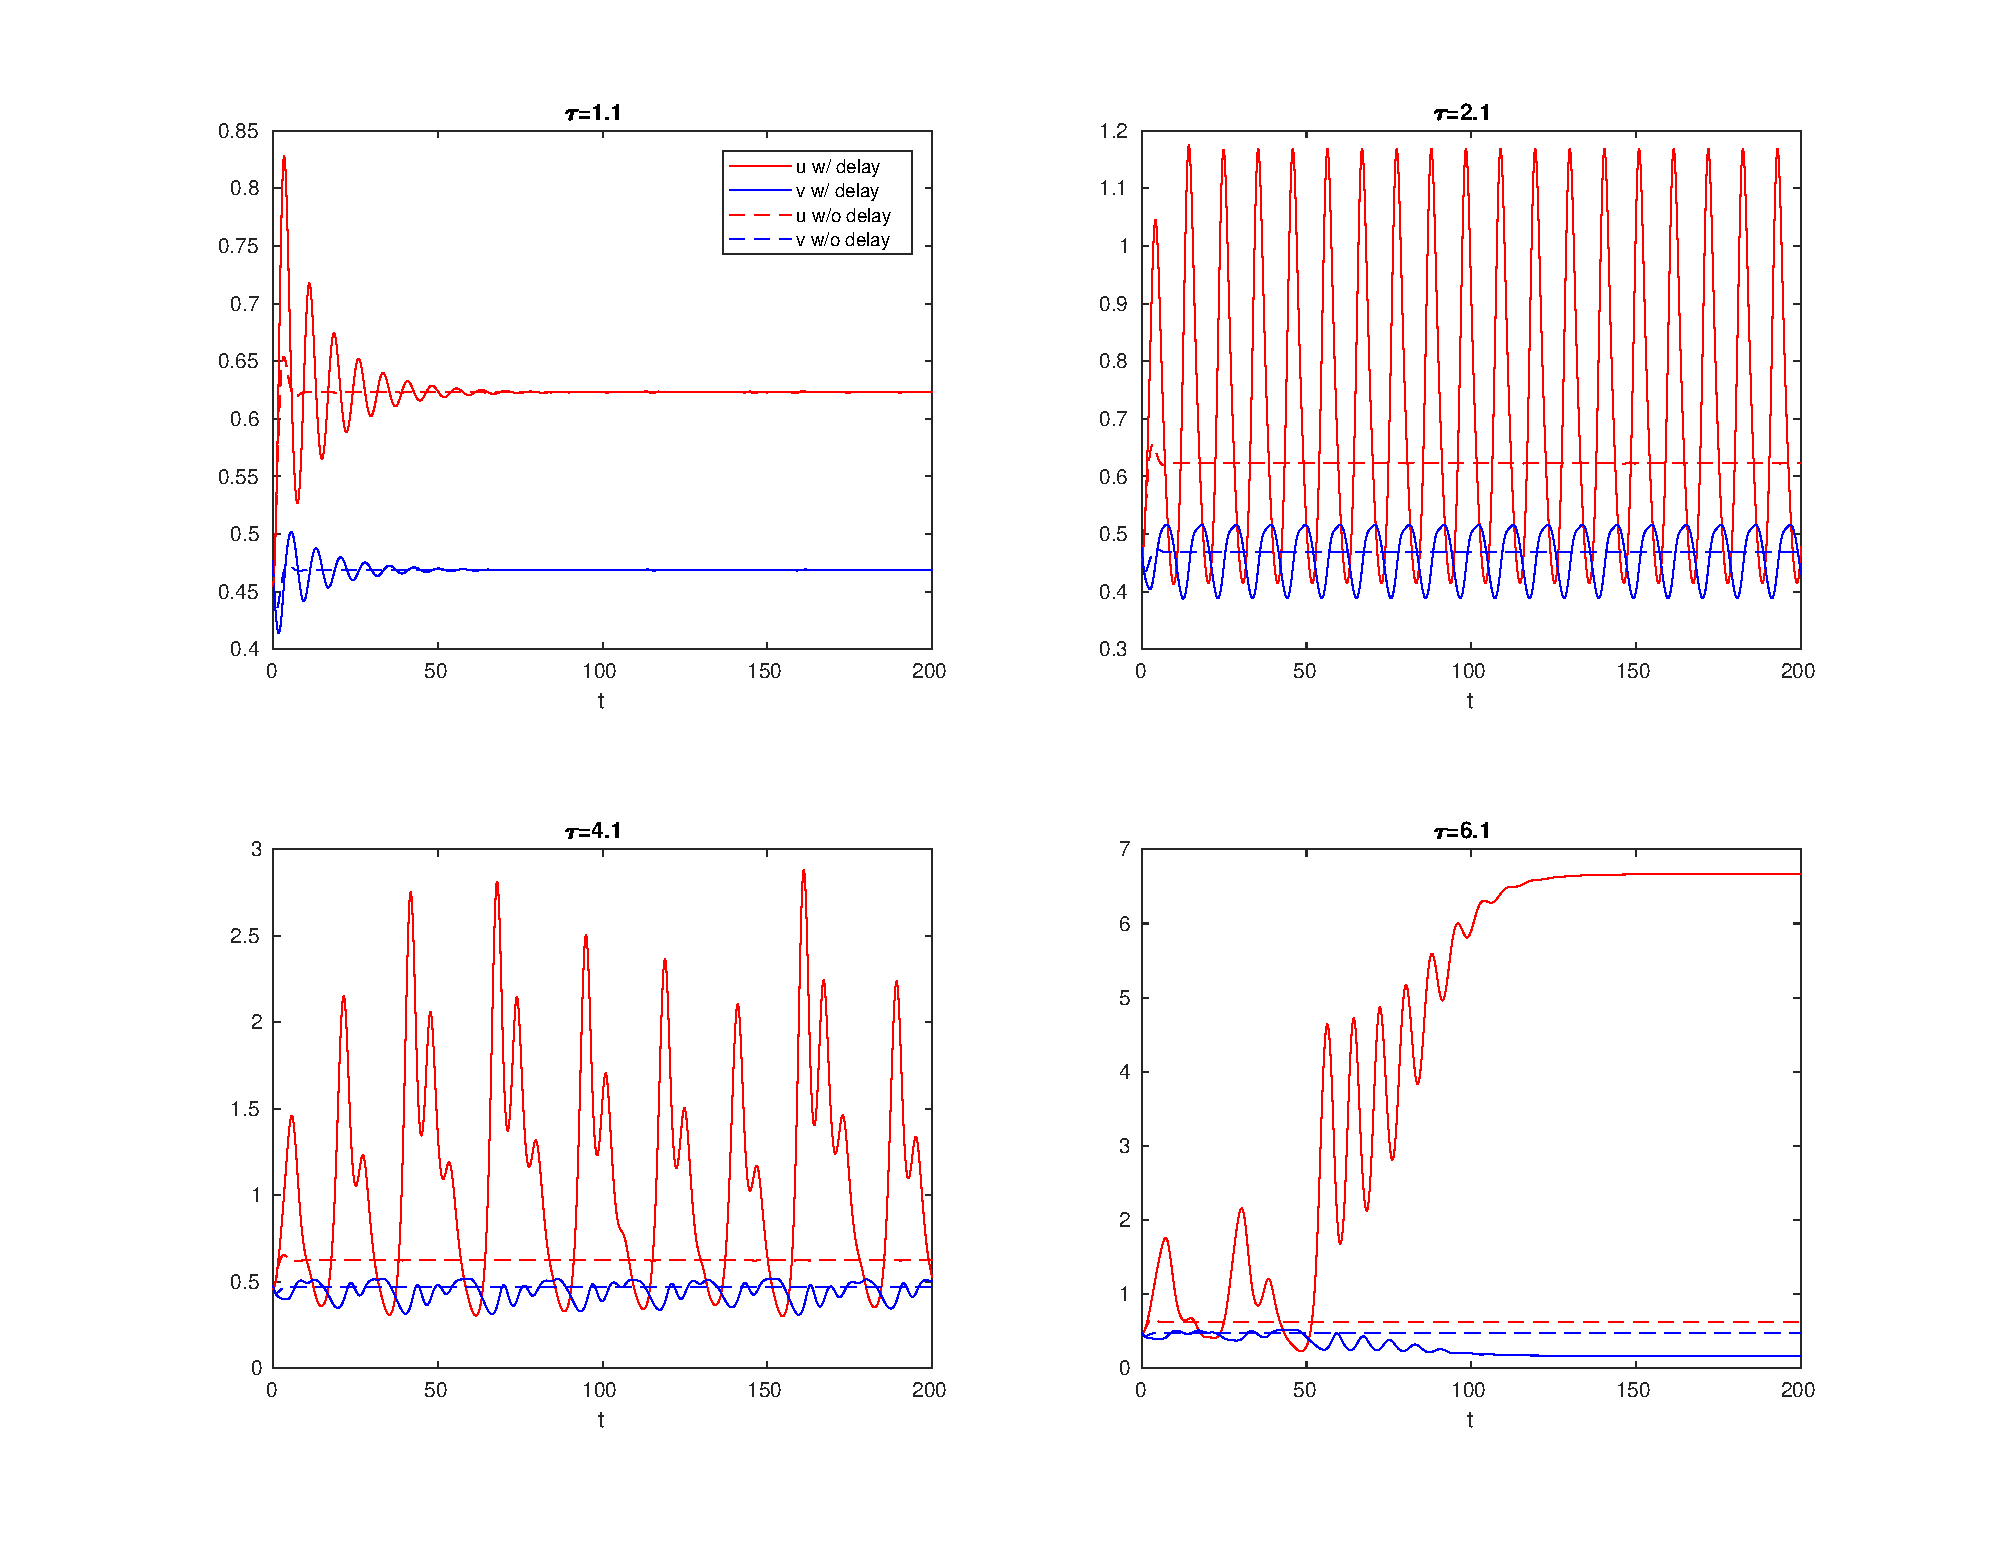
\includegraphics[viewport=70bp 0bp 947bp 818bp,scale=0.4]{explore/plots/varytau/combine}

\caption{\label{fig:stablity switch and shift} Time course of $u$ and $v$ with and without delay.
There is a stability switch as $\tau$ increases and eventually the
solution settles down to high tumor equilibrium. The observation indicates that responsiveness of the immune system is important to contain the tumor in its nascent size. If there is long time delay in immune response, the tumor can grow in oscillatory fashion and eventually escape the control of the immune system.  Parameter values
used to generate the plots: $\rho=2.5,\text{\ensuremath{\beta=0.02,\gamma=5,K=10}}$  }

\end{figure}

% \newpage{}
% 
 \section{With noise}
 
 Tumor cell growth is known to lack of certain regulations compare to normal cells, we thus assume that the innate proliferation rate of tumor cells is subject to uncertainty. Adding white noise to it results
 in the following stochastic differential equations
 
 \begin{subequations}\label{eq:sde}
 \begin{align}
 du & =(\text{\ensuremath{\rho u(1-\frac{u}{K})-\gamma uv)dt+\sigma u(1-\frac{u}{K})dB(t)}},\\
 dv & =(\beta-v+\frac{u}{1+u^{2}})dt.
 \end{align}
 \end{subequations}where $B(t)$ is a scalar Brownian motion defined
 on the complete probability space $(\Omega,\mathcal{F},\{\mathcal{F}_{t}\}_{t\ge0},P)$
 with filtration $\{\mathcal{F}_{t}\}_{t\ge0}$. We use $a\land b$
 to denote min$(a,b)$, $a \lor b$ to denote max$(a,b)$ and a.s. to denote almost surely. 
 
 \subsection{Analysis}
 
 We first show existence and uniqueness of a global solution remains in $\mathcal{D}=(0,K)\times(\beta,\beta+u_{m})$
 where $u_{m}=\max_{u\in(0,K)}\{\frac{u}{1+u^{2}}\}$, whenever it starts in $\mathcal{D}$. Because the drift term and noise term in (\ref{eq:sde}) do not satisfy linear growth condition, the general existence and uniqueness theorem (see \cite{MaoSDEBook} chapter 2) does not apply. The techniques employed here are standard and follow the similar lines as \cite{Wang2017,Gray2011}.
 \begin{theorem}
 \label{thm:exist and unique}For any given initial value $(u(0),v(0))\in\mathcal{D}$,
 there is a unique solution defined for all $t\ge0$, and the solution
 remains in $\mathcal{D}$ a.s.
 \end{theorem}
 
 \begin{proof}
 Since the drift is locally Lipschitz continuous, there is a unique
 local solution on $t\in[0,\tau_{e})$ where $\tau_{e}$ is the explosion
 time, i.e. when the solution exits $\mathcal{D}$. If we can show that $\tau_e=\infty$ a.s., then the solution stays in $\mathcal{D}$ a.s. for all $t>0$.  
 
 Let $\mathcal{D}_{n}=(\frac{1}{n},K-\frac{1}{n})\times(\beta+\frac{1}{n},\beta+u_{m}-\frac{1}{n}$)
 where $n\in\mathbb{N}^{+}$. Define the stopping time 
 \[
 \tau_{n}=\inf\{t\in(0,\tau_{e}):(u(t),v(t))\notin\mathcal{D}_{n}\}.
 \]
 Clearly $\tau_{n}$ increases as $n$. Let $\tau_{\infty}=\lim_{n\to\infty}t_{n}$
 and we have $\tau_{e}\ge\tau_{\infty}$. If we can show that $\tau_{\infty}=\infty$
 a.s., then $\tau_{e}=\infty$ a.s. and we have the unique solution
 $(u(t),v(t))\in\mathcal{D}$ for all $t$.
 
 Suppose on contrary that there is a pair of constants $T>0$ and $\epsilon\in(0,1)$ such that
  $P(\tau_{\infty}\le T)>\text{\ensuremath{\epsilon}}$. Then there
 is a $n_{1}$ such that  $P(\tau_{n}\le T)\ge\epsilon$ for $n>n_{1}$
 . Define $V:\mathcal{D}\to\mathbb{R}$ by
 \begin{equation}
 V(u,v)=\frac{1}{u}+\frac{1}{K-u}+\frac{1}{v-\beta}+\frac{1}{\beta+u_{m}-v},\label{eq:V(u,v)}
 \end{equation}
 where we note it is nonnegative for $u,v\in\mathcal{D}$. 
 
 In general, given an Ito process $dX(t)=b(X(t)dt+\sigma(X_t)dB(t)$ and if $f \in C_0^2(\mathbb{R}^n)$, then $Af(x) = \sum_i b_i(x) \frac{\partial f}{\partial x_i} + \frac{1}{2} \sum_{i,j} (\sigma \sigma^T)_{i,j}(x) \frac{\partial^2 f}{\partial x_i \partial x_j}$ (see Theorem 7.3.3 on Page 126 of \cite{OksendalSDEBook}).
 
 Consider the generator $A$ of (\ref{eq:sde}) and let $A$ act on $V$, i.e., $AV:\mathcal{D}\to\mathbb{R}$.
 Some calculation shows that 
 \begin{eqnarray*}
 AV & = & \begin{pmatrix}\rho u(1-u/K)-\gamma uv\\
 \beta-v+u/(1+u^{2})
 \end{pmatrix}\cdot\begin{pmatrix}-1/u^{2}+1/(K-u)^{2}\\
 -1/(v-\beta)^{2}+1/(\beta+u_{m}-v)^{2}
 \end{pmatrix}\\
  &  & +\frac{\sigma^2}{2}u^{2}(1-\frac{u}{K})^{2}(\frac{2}{u^{3}}+\frac{2}{(K-u)^{3}})\\
  & = & (\gamma v-\rho(1-\frac{u}{K}))\frac{1}{u}+\frac{\rho u}{K}\frac{1}{K-u}-\frac{\gamma uv}{(K-u)^{2}}\\
  &  & +(\beta-v+\frac{u}{1+u^{2}})\frac{1}{(\beta+u_{m}-v)^{2}}+(v-\beta-\frac{u}{1+u^{2}})\frac{1}{(v-\beta)^{2}}\\
  &  & +(1-\frac{u}{K})^{2}\frac{1}{u}+\frac{u^{2}}{K^{2}}\frac{1}{K-u}\\
  & \le & CV,
 \end{eqnarray*}
 where $C=\frac{\rho}{k} \lor \gamma(\beta+u_m) \lor (\gamma(\beta+u_m)+1)$ a positive constant. By Dynkin's
 formula (see, e.g., \cite{OksendalSDEBook} Page 127), we have 
 \begin{eqnarray*}
 E[V(u(\tau_{n}\land T),v(\tau_{n}\land T))] & = & V(u(0),v(0))+E[\int_{0}^{\tau_{n}\land T}AV(u(s),v(s)ds]\\
  & \le & V(u(0),v(0))+C\int_{0}^{T}E[V]ds.
 \end{eqnarray*}
 By Gronwall's inequality, 
 \begin{eqnarray*}
 E[V(u(\tau_{n}\land T),v(\tau_{n}\land T))] & \le & V(u(0),v(0))e^{CT}<\infty.
 \end{eqnarray*}
 On the other hand, consider the set $\Omega_{n}=\{\tau_{n}\le T\}$
 for $n>n_{1}$ for which we know $P(\Omega_{n})\ge\epsilon$. For
 $\omega\in\Omega_{n}$, we know that $V\sim O(n)$. Thus 
 \begin{eqnarray*}
 E[V(u(\tau_{n}\land T),v(\tau_{n}\land T))] & \ge & E[\boldsymbol{1}_{\Omega_{n}}V(u(\tau_{n}\land T),v(\tau_{n}\land T))]\\
  & = & \epsilon V(u(\tau_{n},\omega),v(\tau_{n},\omega))\to\infty,
 \end{eqnarray*}
 if we let $n\to\infty$. Hence we have a contradiction. 
 \end{proof}
 Having established existence and uniqueness of a global solution, we present
 a theorem regarding to tumor extinction. Its proof involves an application of Ito's formula (see, e.g., \cite{OksendalSDEBook} Page 49) to show $\limsup_{t\to\infty}\frac{1}{t}\log(u(t))<0\text{ a.s.}$, namely, the tumor population tends to zero exponentially a.s..   
 \begin{theorem}
 \label{thm:(tumor-extinction)}\textup{(tumor extinction)} If one
 of the conditions holds 
 
 i) $\sigma^{2}>\rho\vee\frac{\rho^{2}}{2\gamma\beta}$
 
 ii) $\sigma^{2}<\rho<\sigma^{2}/2+\gamma\beta$
 
 then for $(u(0),v(0))\in\mathcal{D}$
 \[
 \limsup_{t\to\infty}\frac{1}{t}\log(u(t))<0\text{ a.s.}
 \]
 \end{theorem}
 
 \begin{proof}
 By Ito's formula, we have 
 \begin{eqnarray*}
 \log(u(t)) & = & \log(u_{0})+\int_{0}^{t}\rho(1-\frac{u(s)}{K})-\gamma v(s)-\frac{\sigma^{2}}{2}(1-\frac{u(s)}{K})^{2}ds\\
  &  & +\int_{0}^{t}\sigma(1-\frac{u(s)}{K})dB(s)\\
  & \le & \log(u_{0})+\int_{0}^{t}f(1-\frac{u(s)}{K})ds+\int_{0}^{t}\sigma(1-\frac{u(s)}{K})dB(s)
 \end{eqnarray*}
 where $f(y)=-\frac{1}{2}\sigma^{2}y^{2}+\rho y-\gamma\beta$. Note that $f(y)$ is a concave-down quadratic function with axis of symmetry $y=\frac{\rho}{\sigma^2}$ and $y(0)<0$. There are two ways to ensure $\max_{y\in(0,1)} f(y)<0$, i.e., 
 
\begin{eqnarray*}
\begin{cases}
\frac{\rho}{\sigma^{2}}<1\\
f(\frac{\rho}{\sigma^{2}})<0,
\end{cases}
 & \text{or \  \ } & \begin{cases}
\frac{\rho}{\sigma^{2}}>1\\
f(1)<0
\end{cases}
\end{eqnarray*} 
which corresponds to the stated conditions i) or ii).
 Thus, 
 \begin{eqnarray*}
 \limsup_{t\to\infty}\frac{1}{t}\log(u(t)) & \le & \max_{y\in(0,1)}f(y)+\limsup_{t\to\infty}\frac{1}{t}\int_{0}^{t}\sigma(1-\frac{u(s)}{K})dB(s),\\
  & < & 0\text{ a.s.}
 \end{eqnarray*}
 where the term with integral is zero a.s. by law of large numbers
 of martingale (see, e.g., \cite{MaoSDEBook}). 
 \end{proof}
 To complement with the condition for tumor extinction, we present
 a theorem for tumor persistence in the following. The proof involves construction of a contradiction to show that $\limsup_{t\to\infty}u(t)$ is bounded from below, and again Ito's formula is the workhorse behind this type of proof. 
 \begin{theorem}
 \label{thm:stoch-persistence}\textup{(tumor persistence)} If $\rho>\sigma^{2}/2+\gamma(\beta+u_{m})$,
 then for any given initial value $(u(0),v(0))\in\mathcal{D}$, we
 have 
 \[
 \limsup_{t\to\infty}u(t)>\xi
 \]
  a.s. where $\xi$ is the positive root of $g(u)=-\frac{1}{2}\sigma^{2}(1-\frac{u}{K})^{2}+\rho(1-\frac{u}{K})-\gamma(\beta+u_{m})$. 
 \end{theorem}
 
 \begin{proof}
 Assume $\rho>\sigma^{2}/2+\gamma(\beta+u_m)$. We note that $g(K)<0$
 and $g(0)=-\frac{1}{2}\sigma^{2}+\rho-\gamma(\beta+u_{m})>0$. Thus
 $\xi$ exists and $g'(u)<0$ for $u$ in a small neighborhood of $\xi$.
 Suppose on contrary that there is a small $\epsilon\in(0,1)$ such that $P(\Omega_{1})>\epsilon$ where $\Omega_{1}=\{\omega: \limsup_{t\to\infty} u(t,\omega)<\text{\ensuremath{\xi-2\epsilon}}\}$.
 Then there is $T(\omega)>0$ such that  
 \begin{equation}
 u(t,\omega)<\xi-\epsilon\text{ for }t>T(\omega).\label{eq:u<xi-esp}
 \end{equation}
  We choose $\epsilon$ small enough so that $g(u(t,\omega)>g(\xi-\epsilon)$
 for $t>T(\omega)$. Moreover, by law of large numbers of martingale
 there is $\Omega_{2}\subset\Omega$ with $P(\Omega_{2})=1$ such that
  for any $\omega\in\Omega_{2}$, $\lim_{t\to\infty}\frac{1}{t}\int_{0}^{t}\sigma(1-\frac{u(s)}{K})dB(s,\omega)=0$.
 
 Now considering $\omega\in\Omega_{1}\cap\Omega_{2}$, we have
 \begin{eqnarray*}
 \log(u(t,\omega)) & \ge & \log(u_{0})+\int_{0}^{t}g(u(s))ds+\int_{0}^{t}\sigma(1-\frac{u(s)}{K})dB(s,\omega)\\
  & \ge & \log(u_{0})+\int_{0}^{T(\omega)}g(u(s)ds+(t-T(\omega))g(\xi-\epsilon)\\
  &  & +\int_{0}^{t}\sigma(1-\frac{u(s)}{K})dB(s,\omega).
 \end{eqnarray*}
 Thus we have 
 \begin{eqnarray*}
 \liminf_{t\to\infty}\frac{1}{t}\log(u(t,\omega)) & \ge & g(\xi-\epsilon)>0,
 \end{eqnarray*}
 which implies that $u(t,\omega)\to\infty$, which contradicts (\ref{eq:u<xi-esp}). 
 \end{proof}
 We compare the conditions in the previous two theorems to their counterparts
 in section 3. In the original units, we find two noise magnitude regimes
 with $\frac{\hat{\rho}}{\hat{\mu}}$ as the threshold (we call $\sigma^{2}<\frac{\hat{\rho}}{\hat{\mu}}$
 small noise regime and $\sigma^{2}>\frac{\hat{\rho}}{\hat{\mu}}$ big noise regime).
 In the small noise regime, the tumor extinction condition is weaker
 than the one for the deterministic system. The biological interpretation
 is that the small noise can possibly help eliminate the tumor. The
 condition for tumor persistence is stronger in the stochastic system.
 However, it is only a sufficient condition and there is a gap between
 between the persistence condition and the extinction condition. 
 
 \subsection{Numerical simulation}
 
 (\ref{eq:sde}) is simulated using Milstein\textquoteright s method
 \cite{Higham.2001}. As in Figure \ref{fig:noise}, the simulation
 confirmed our extinction criteria. Also shown is that the tumor persists
 in the monostability where the solution simply fluctuates about the
 equilibrium and bistablity where there is a noise-induced transition
 to high tumor equilibrium from low tumor equilibrium. The parameter
 values used in the simulations are summarized in Table  \ref{tab:parameter-values}. 
 
 \begin{table}
 \begin{tabular}{c>{\centering}m{0.12\paperwidth}>{\centering}m{0.12\paperwidth}>{\centering}m{0.12\paperwidth}>{\centering}m{0.12\paperwidth}}
 \toprule 
  & small noise induced extinction (a) & big noise induced extinction (b) & monostable (c) & bistable (d)\tabularnewline
 \midrule
 \midrule 
 $\rho$ & 0.12 & 2.5 & 1.5 & 2.5\tabularnewline
 \midrule 
 $\beta$ & 0.02 & 0.02 & 0.02 & 0.02\tabularnewline
 \midrule 
 $\gamma$ & 5 & 5 & 5 & 5\tabularnewline
 \midrule 
 $K$ & 10 & 10 & 10 & 10\tabularnewline
 \midrule 
 $\sigma$ & 0.3 & 5.66 & 0.65 & 0.65\tabularnewline
 \bottomrule
 \end{tabular}
 
 \caption{\label{tab:parameter-values}Parameter values used in Figure \ref{fig:noise}}
 \end{table}
 
 \begin{figure}
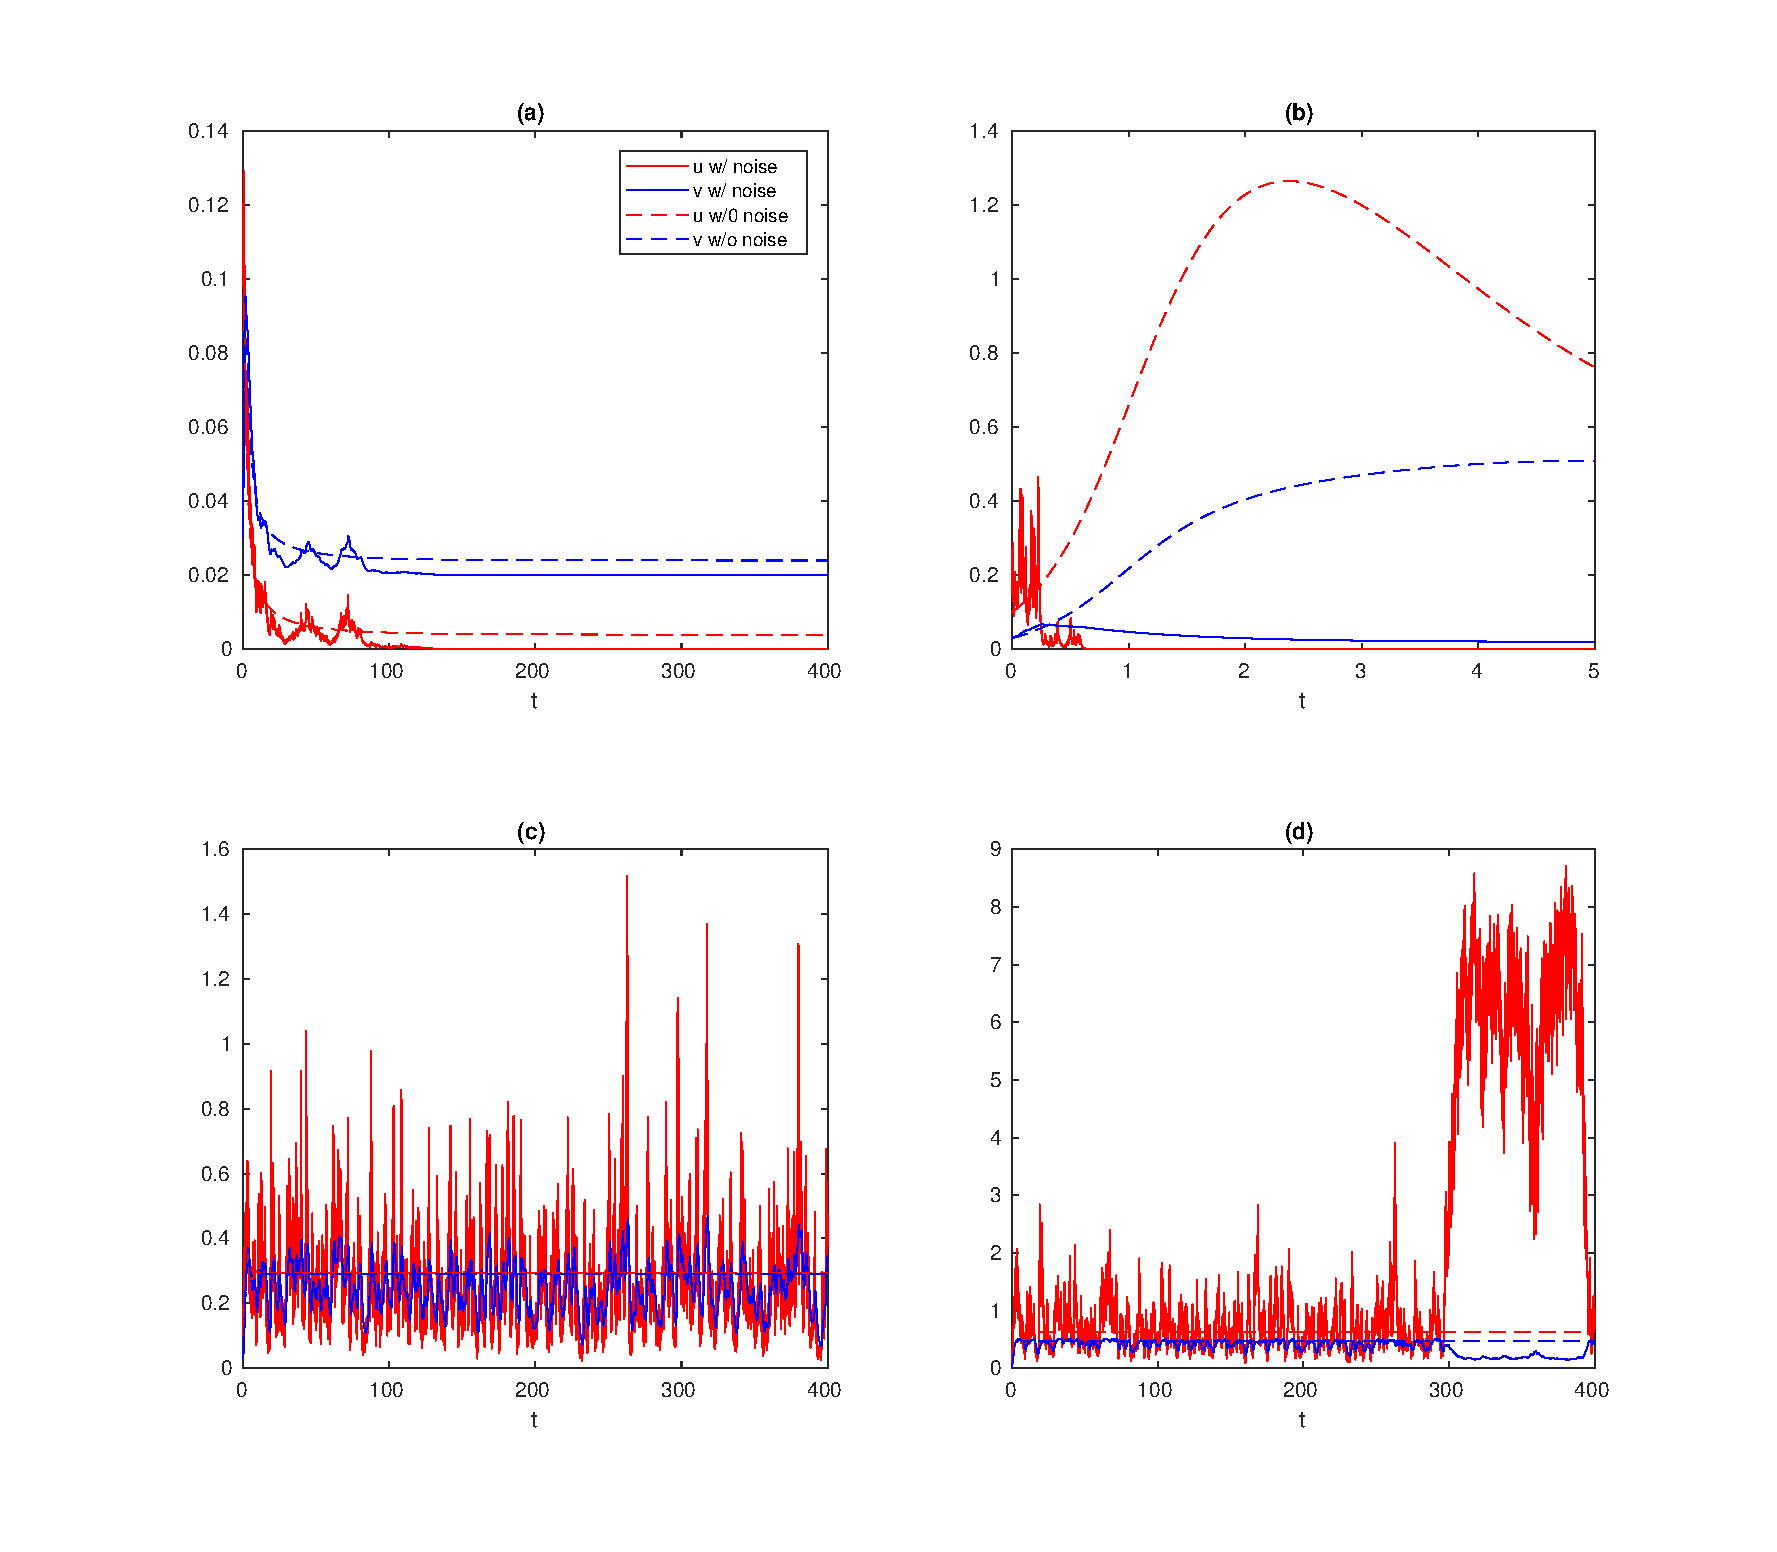
\includegraphics[scale=0.4]{explore/plots/sde-extinction-switch/sde-extinction-switch.eps} 
 \caption{\label{fig:noise}Computer simulated sample paths of the stochastic
 system (\ref{eq:sde}) in comparison with its deterministic version
 (\ref{eq: uv }). (a) tumor extinction in small noise regime; (b)
 tumor extinction in big noise regime; (c) monostable fluctuation;
 (d) bistable switching. Parameter values used here are summarized
 in Table \ref{tab:parameter-values} }
 
 \end{figure}
% 
% \newpage{}
% 
 \section{With delay and noise}
 
 In this section, we study the system when both delay and noise are
 present as follows
 
 \begin{subequations}\label{eq: sdde}
 \begin{align}
 du & =(\text{\ensuremath{\rho u(1-\frac{u}{K})-\gamma uv)dt+\sigma u(1-\frac{u}{K})dB(t)}},\\
 dv & =(\beta-v+\frac{u(t-\tau)}{1+u(t-\tau)^{2}})dt.
 \end{align}
 \end{subequations}
 
 \subsection{Analysis}
 
 The analysis in section 4 can be extended
 to (\ref{eq: sdde}). Because of the time delay $\tau$, here we need
 to supply suitable initial data on $[-\tau,0]$. The extension of
 Theorem \ref{thm:exist and unique} is stated as follows 
 \begin{theorem}
 For any initial data $\{(u(t),v(t)):-\tau\le t\le0\}\in C([-\tau,0],\mathcal{D})$,
 there is a unique solution defined for all $t\ge-\tau$ and remains
 in $\mathcal{D}$ a.s.
 \end{theorem}
 
 \begin{proof}
 The proof follows similar lines as the one for Theorem \ref{thm:exist and unique} with
 an application of method of steps. We keep the same definition of
 $\tau_{n},\tau_{\infty},\tau_{e}$ and $V(u,v)$. Same as before we
 want to show that $\tau_{e}=\infty$ by proving that $\tau_{\infty}=\infty$.
 First we want to show that $\tau_{\infty}>\tau$. For any $n\in\mathbb{N}^{+}$
 and $t\in[0,\tau_{\infty})$, it can be shown by Ito formula that
 \begin{equation}
 dV(u(t),v(t))=LV(u(t),v(t),u(t-\tau),v(t-\tau))+\sigma(\frac{u}{K(K-u)}+\frac{1}{K}-\frac{1}{u})dB(t)\label{eq:dV delay}
 \end{equation}
 where 
 \begin{align*}
  & LV(u(t),v(t),u(t-\tau),v(t-\tau))\\
 = & [\gamma v-\rho(1-\frac{u}{K})+(1-\frac{u}{K})^{2}]\frac{1}{u}+[\frac{\rho u}{K}+\frac{u^{2}}{K^{2}}]\frac{1}{K-u}+\frac{1}{\beta+u_{m}-v}+\frac{1}{v-\beta}\\
  & -[u_{m}-\frac{u(t-\tau)}{1+u(t-\tau)^{2}}]\frac{1}{(\beta+u_{m}-v)^{2}}-[\frac{u(t-\tau)}{1+u(t-\tau)^{2}}]\frac{1}{(\beta-v)^{2}}\\
 \le & K_{1}V
 \end{align*}
 where $K_{1}$ is a positive constant. For $t_{1}\in[0,\tau]$, integrating
 (\ref{eq:dV delay}) from 0 to $t_{1}\land\tau_{n}$ and taking expectation
 gives
 \begin{eqnarray*}
 E[V(u(t_{1}\land\tau_{n}),v(t_{1}\land\tau_{n})] & \le & V(u(0),v(0))+\int_{0}^{t_{1}\land\tau_{n}}V(u(s),v(s))ds
 \end{eqnarray*}
 By Gronwall's inequality, $E[V(u(t_{1}\land\tau_{n}),v(t_{1}\land\tau_{n})]\le V(u(0),v(0))e^{\tau}<\infty$.
 In particular, 
 \begin{equation}
 E[V(u(\tau\land\tau_{n}),v(\tau\land\tau_{n})]\le V(u(0),v(0))e^{\tau}<\infty.\label{eq:EV<inf}
 \end{equation}
 Suppose on contrary there is $\epsilon>0$ such that $P(\tau_{\infty}<\tau)>\epsilon$.
 Then there is $n_{1}$ such that for $n>n_{1}$, $P(\Omega_{1})\ge\epsilon$
 where $\Omega_{1}=\{\omega:\tau_{n}(\omega)<\tau\}$. Thus 
 \begin{eqnarray*}
 E[V(u(\tau\land\tau_{n}),v(\tau\land\tau_{n})] & \ge & E[\boldsymbol{1}_{\Omega_{1}}V(u(\tau_{n}),v(\tau_{n})]\\
  & \ge & \epsilon n\to\infty
 \end{eqnarray*}
 as $n\to\infty$, which is a contradiction to \ref{eq:EV<inf}. Thus
 for $\tau_{\infty}\ge\tau$. By the same argument on $t\in[\tau,2\tau],$we
 have $\tau_{\infty}\ge2\tau$. Repeating this procedure gives $\tau_{\infty}=\infty$. 
 \end{proof}
It is easy to see that $v(t)\in(\beta,\beta+\frac{1}{2})$ for all $t>0$.
 This enables Theorem \ref{thm:(tumor-extinction)} and Theorem \ref{thm:stoch-persistence}
 be extended to the system (\ref{eq: sdde}) with similar arguments. 
 
 \subsection{Numerical simulation}
 
 From previous analysis, we notice that the system (\ref{eq: sdde})
 bears a lot of similarity to the system (\ref{eq:sde}). In this subsection,
 we instead focus on the effect of time delay on stationary distributions
 by numerical simulations. As seen in Figure \ref{fig:statdistr},
 the stationary distribution is bimodal which is not a surprise since
 the underlying deterministic system is bistable. As the delay increases (larger
 $\tau$), the more density shifts to the high tumor stable state and
 the bimodality becomes indistinguishable at $\tau=2$. We also observe
 that the mean first passage time from the low tumor stable state to
 the high tumor stable state is reduced by increasing $\tau$.
 
 \begin{figure}
 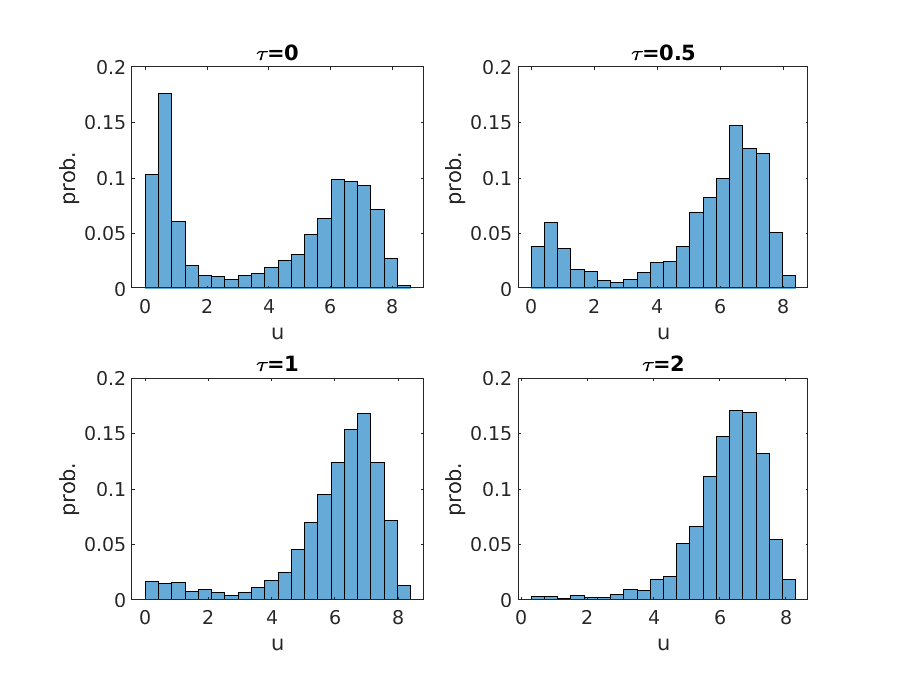
\includegraphics[scale=0.8]{explore/plots/statdist/statdist}
 
 \caption{\label{fig:statdistr}stationary distribution of (\ref{eq: sdde})
 with $\tau=0,0.5,1,2$. The histogram is formed by 5000 samples of
 $u(1000)$. }
 \end{figure}
 
 
 \section{Discussion and conclusion.}
 
 In this paper, we presented a simple model of tumor-immune system
 interactions, in which the immune response to tumor is modeled as
 a non-monotonic function of tumor burden. We studied the effects of
 time delay in the immune response and the uncertainty in the innate
 proliferating rate of cancer cells on the tumor growth dynamics. The
 conditions of tumor extinction and persistence were proved in presence
 of noise or time delay. We also performed numerical experiments to
 confirm analytical results and to guide future analytical work. 
 
 We showed that the magnitude of the tumor reproduction number $R_0=\frac{\hat{\mu}\hat{\rho}}{\hat{\gamma}\hat{\beta}}$
 relative to 1 dictates the stability of tumor-free equilibrium. This
 condition does not depend on time delay. It suggests that the elimination of cancer depends on the basal level of the immune system rather than on its response speed to tumor growth. However, it maybe possible to have delay-induced stability switching for the low-tumor steady state. 
 We also established the global stability of tumor-free equilibrium,
 but that of interior equilibria is challenging and remains an open
 problem. 
 
 For stochastic version of the model, we showed that the noise can
 help eliminate cancer in either case of big or small noise. Similar
 results in an epidemic model were obtained by \cite{Gray2011}. We
 note that the criteria for persistence in Theorem \ref{thm:stoch-persistence}
 is not a necessary condition and in fact far from being a sharp result.
 Indeed, parameter sets (c) (d) do not satisfy the persistence condition
 but appear to be persistent in the numerical simulation. The improvement
 of the current result will be deferred to future work. Also, as seen
 in the simulation, there is a stationary distribution of (\ref{eq:sde}).
 However, it is challenging to show this analytically because the diffusion
 matrix is degenerate, which makes the standard techniques employed
 in \cite{Wang2017,Gray2011} not applicable. There have been recent
 studies on the stationary distribution resulting from a degenerate
 diffusion matrix \cite{Lan2018}. It will also be the focus of our
 future work. 
 
 When including time delay with noise, we showed that the results we
 obtained for noise-only system (\ref{eq:sde}) can be easily extended
 to (\ref{eq: sdde}). Moreover, we found numerically that the noise
 favors transition to high tumor stable state, which was also observed
 for an ecological model studied in \cite{Zeng2012}. The biological
 implication is that the less responsive the immune system is, the
 easier for the tumor to escape to high burden. Same as for the noise-only
 version of the model, the existence of a stationary distribution of (\ref{eq: sdde}) will
 be the focus of future work. There are some perturbation techniques
 applied to delayed Focker-Planck equation to study the effects of
 time delay on mean first passage time \cite{Kuchler1992,Guillouzic1999,Frank2005}.
 Those techniques are limited to a scalar equation. Possible extension
 to study a system of equations will be carried out in the future. 
 
 Time delay and stochasticity are two hallmarks of cancer dynamics.
 Serious modeling work shall not shy away from them. The model we studied
 was kept minimal but nevertheless exhibited interesting dynamics.
 It is hoped that this paper will stimulate interests in stochastic
 delayed differential equations in modeling cancer dynamics. 
 
\section*{Acknowledgments.}
 The authors would like to thank Professor Hal Smith for helpful discussions.
% 
%\bibliographystyle{AIMS}
% \nocite{*}
% \bibliography{DDEs-TANTs-new}

\providecommand{\href}[2]{#2}
\providecommand{\arxiv}[1]{\href{http://arxiv.org/abs/#1}{arXiv:#1}}
\providecommand{\url}[1]{\texttt{#1}}
\providecommand{\urlprefix}{URL }
\begin{thebibliography}{10}

\bibitem{Banerjee2008}
\newblock S.~Banerjee and R.~R. Sarkar,
\newblock {Delay-induced model for tumor-immune interaction and control of
  malignant tumor growth},
\newblock \emph{Biosystems}, \textbf{91} (2008), 268--288,
\newblock
  \urlprefix\url{https://www.sciencedirect.com/science/article/pii/S0303264707001499}.

\bibitem{Bose2009}
\newblock T.~Bose and S.~Trimper,
\newblock {Stochastic model for tumor growth with immunization},
\newblock \emph{Physical Review E}, \textbf{79} (2009), 051903,
\newblock \urlprefix\url{https://link.aps.org/doi/10.1103/PhysRevE.79.051903}.

\bibitem{dOnofrio2008}
\newblock A.~D'Onofrio,
\newblock {Metamodeling tumor-immune system interaction, tumor evasion and
  immunotherapy},
\newblock \emph{Mathematical and Computer Modelling}, \textbf{47} (2008),
  614--637,
\newblock
  \urlprefix\url{https://www.sciencedirect.com/science/article/pii/S0895717707001951}.

\bibitem{dOnofrio2010}
\newblock A.~D'Onofrio, F.~Gatti, P.~Cerrai and L.~Freschi,
\newblock {Delay-induced oscillatory dynamics of tumour-immune system
  interaction},
\newblock \emph{Mathematical and Computer Modelling}, \textbf{51} (2010),
  572--591,
\newblock
  \urlprefix\url{https://www.sciencedirect.com/science/article/pii/S089571770900404X}.

\bibitem{Eftimie2011}
\newblock R.~Eftimie, J.~L. Bramson and D.~J.~D. Earn,
\newblock {Interactions between the immune system and cancer: A brief review
  of non-spatial mathematical models},
\newblock \emph{Bulletin of Mathematical Biology}, \textbf{73} (2011), 2--32,
\newblock \urlprefix\url{http://link.springer.com/10.1007/s11538-010-9526-3}.

\bibitem{fisher2013cancer}
\newblock R.~Fisher, L.~Pusztai and C.~Swanton,
\newblock {Cancer heterogeneity: implications for targeted therapeutics},
\newblock \emph{British journal of cancer}, \textbf{108} (2013), 479.

\bibitem{Frank2005}
\newblock T.~D. Frank,
\newblock {Delay Fokker-Planck equations, perturbation theory, and data
  analysis for nonlinear stochastic systems with time delays},
\newblock \emph{Physical Review E}, \textbf{71} (2005), 031106,
\newblock
  \urlprefix\url{https://journals.aps.org/pre/abstract/10.1103/PhysRevE.71.031106}.

\bibitem{galach2003dynamics}
\newblock M.~Ga{\l}ach,
\newblock {Dynamics of the tumor--immune system competition---the effect of
  time delay},
\newblock \emph{International Journal of Applied Mathematics and Computer
  Science}, \textbf{13} (2003), 395--406,
\newblock
  \urlprefix\url{https://pdfs.semanticscholar.org/88fb/d5af40f9ebdba3e4d262b0d5bf80963199b4.pdf}.

\bibitem{Gray2011}
\newblock A.~Gray, D.~Greenhalgh, L.~Hu, X.~Mao and J.~Pan,
\newblock {A stochastic differential equation SIS epidemic model},
\newblock \emph{SIAM Journal on Applied Mathematics}, \textbf{71} (2011),
  876--902,
\newblock \urlprefix\url{http://epubs.siam.org/doi/10.1137/10081856X}.

\bibitem{Guillouzic1999}
\newblock S.~Guillouzic, I.~L'Heureux and A.~Longtin,
\newblock {Small delay approximation of stochastic delay differential
  equations},
\newblock \emph{Physical Review E}, \textbf{59} (1999), 3970--3982,
\newblock \urlprefix\url{https://link.aps.org/doi/10.1103/PhysRevE.59.3970}.

\bibitem{Guo2014}
\newblock W.~Guo and D.-C. Mei,
\newblock {Stochastic resonance in a tumor-immune system subject to bounded
  noises and time delay},
\newblock \emph{Physica A: Statistical Mechanics and its Applications},
  \textbf{416} (2014), 90--98,
\newblock
  \urlprefix\url{https://www.sciencedirect.com/science/article/pii/S0378437114006748}.

\bibitem{Higham.2001}
\newblock D.~J. Higham.,
\newblock {An algorithmic introduction to numerical simulation of stochastic
  differential equations},
\newblock \emph{SIAM Review}, \textbf{43} (2001), 525--546,
\newblock \urlprefix\url{http://epubs.siam.org/doi/10.1137/S0036144500378302}.

\bibitem{Kirschner1998}
\newblock D.~Kirschner and J.~C. Panetta,
\newblock {Modeling immunotherapy of the tumor - immune interaction},
\newblock \emph{Journal of Mathematical Biology}, \textbf{37} (1998), 235--252,
\newblock \urlprefix\url{http://link.springer.com/10.1007/s002850050127}.

\bibitem{KuangDDEBook}
\newblock Y.~Kuang,
\newblock \emph{{Delay Differential Equations with Applications in Population Dynamics}}.
\newblock Academic Press, 1993.

\bibitem{KuangOncologyBook}
\newblock Y.~Kuang, J.~D. Nagy and S.~E. Eikenberry,
\newblock \emph{{Introduction to Mathematical Oncology}}.
\newblock CRC Press, 2016.

\bibitem{MaoSDEBook}
\newblock X.~Mao,
\newblock \emph{{Stochastic Differential Equations and Applications}}, 
\newblock Elsevier, 2007.

\bibitem{OksendalSDEBook}
\newblock B.~{\O}ksendal,
\newblock \emph{{Stochastic Differential Equations}}, 
\newblock Springer, 2003.

\bibitem{Kuchler1992}
\newblock U.~K{\"{u}}chler and B.~Mensch,
\newblock {Langevins stochastic differential equation extended by a
  time-delayed term},
\newblock \emph{Stochastics and Stochastic Reports}, \textbf{40} (1992),
  23--42,
\newblock
  \urlprefix\url{https://www.tandfonline.com/doi/full/10.1080/17442509208833780}.

\bibitem{Kuznetsov1994}
\newblock V.~A. Kuznetsov, I.~A. Makalkin, M.~A. Taylor and A.~S. Perelson,
\newblock {Nonlinear dynamics of immunogenic tumors: Parameter estimation and
  global bifurcation analysis},
\newblock \emph{Bulletin of Mathematical Biology}, \textbf{56} (1994),
  295--321,
\newblock
  \urlprefix\url{https://www.sciencedirect.com/science/article/pii/S0092824005802605}.

\bibitem{Lai2017}
\newblock X.~Lai and A.~Friedman,
\newblock {Combination therapy of cancer with cancer vaccine and immune
  checkpoint inhibitors: A mathematical model},
\newblock \emph{PLOS ONE}, \textbf{12} (2017), e0178479,
\newblock \urlprefix\url{https://dx.plos.org/10.1371/journal.pone.0178479}.

\bibitem{Lan2018}
\newblock G.~Lan, Z.~Chen, C.~Wei and S.~Zhang,
\newblock {Stationary distribution of a stochastic SIQR epidemic model with
  saturated incidence and degenerate diffusion},
\newblock \emph{Physica A: Statistical Mechanics and its Applications},
  \textbf{511} (2018), 61--77,
\newblock
  \urlprefix\url{https://www.sciencedirect.com/science/article/pii/S0378437118309130}.

\bibitem{Lefever1979}
\newblock R.~Lefever and W.~Horsthemke,
\newblock {Bistability in fluctuating environments. Implications in tumor
  immunology},
\newblock \emph{Bulletin of Mathematical Biology}, \textbf{41} (1979),
  469--490,
\newblock
  \urlprefix\url{https://www.sciencedirect.com/science/article/pii/S0092824079800038}.

\bibitem{Li2017}
\newblock D.~Li and F.~Cheng,
\newblock {Threshold for extinction and survival in stochastic tumor immune
  system},
\newblock \emph{Communications in Nonlinear Science and Numerical Simulation},
  \textbf{51} (2017), 1--12,
\newblock
  \urlprefix\url{https://www.sciencedirect.com/science/article/pii/S1007570417300850}.

\bibitem{mahoney2015next}
\newblock K.~M. Mahoney, G.~J. Freeman and D.~F. McDermott,
\newblock {The next immune-checkpoint inhibitors: PD-1/PD-L1 blockade in
  melanoma},
\newblock \emph{Clinical therapeutics}, \textbf{37} (2015), 764--782.

\bibitem{murraymathematical}
\newblock J.~D. Murray,
\newblock {Mathematical Biology: I. An Introduction}.
\newblock Springer, 2002.

\bibitem{Nikolopoulou2018}
\newblock E.~Nikolopoulou, L.~R. Johnson, D.~Harris, J.~D. Nagy, E.~C. Stites
  and Y.~Kuang,
\newblock {Tumour-immune dynamics with an immune checkpoint inhibitor},
\newblock \emph{Letters in Biomathematics}, \textbf{5} (2018), S137--S159,
\newblock
  \urlprefix\url{http://www.tandfonline.com/action/journalInformation?journalCode=tlib20
  https://www.tandfonline.com/doi/full/10.1080/23737867.2018.1440978}.

\bibitem{parish2003cancer}
\newblock C.~R. Parish,
\newblock {Cancer immunotherapy: the past, the present and the future},
\newblock \emph{Immunology and cell biology}, \textbf{81} (2003), 106--113.

\bibitem{Rihan2014}
\newblock F.~Rihan, D.~{Abdel Rahman}, S.~Lakshmanan and A.~Alkhajeh,
\newblock {A time delay model of tumour-immune system interactions: Global
  dynamics, parameter estimation, sensitivity analysis},
\newblock \emph{Applied Mathematics and Computation}, \textbf{232} (2014),
  606--623,
\newblock
  \urlprefix\url{https://www.sciencedirect.com/science/article/pii/S0096300314001568}.

\bibitem{Wang2017}
\newblock L.~Wang, D.~Jiang, G.~S.~K. Wolkowicz and D.~O'Regan,
\newblock {Dynamics of the stochastic chemostat with Monod-Haldane response
  function},
\newblock \emph{Scientific Reports}, \textbf{7} (2017), 13641,
\newblock \urlprefix\url{http://www.nature.com/articles/s41598-017-13294-3}.

\bibitem{Whiteside2006}
\newblock T.~L. Whiteside,
\newblock {Immune suppression in cancer: Effects on immune cells, mechanisms
  and future therapeutic intervention},
\newblock \emph{Seminars in Cancer Biology}, \textbf{16} (2006), 3--15,
\newblock
  \urlprefix\url{https://www.sciencedirect.com/science/article/pii/S1044579X0500060X?via{\%}3Dihub}.

\bibitem{Zeng2012}
\newblock C.~Zeng and H.~Wang,
\newblock {Noise and large time delay: Accelerated catastrophic regime shifts
  in ecosystems},
\newblock \emph{Ecological Modelling}, \textbf{233} (2012), 52--58,
\newblock
  \urlprefix\url{https://www.sciencedirect.com/science/article/pii/S030438001200141X}.

\end{thebibliography}


\end{document}
